\documentclass[a4paper]{scrartcl}
\usepackage[english]{babel}
\usepackage[top=2cm,bottom=3cm,left=2.5cm,right=2.5cm]{geometry}
\usepackage[colorlinks=true, allcolors=black]{hyperref}
\usepackage{wrapfig} %문단 내 이미지 삽입
\usepackage{graphicx} %색상
\usepackage{overpic}
\usepackage[normalem]{ulem}%취소선
\usepackage{array} %표
\usepackage{mdframed, tcolorbox} %글상자
\usepackage[yyyymmdd]{datetime}
	\renewcommand{\dateseparator}{--}
\usepackage{amsmath, amsfonts, amssymb, bm} %수식
	\DeclareMathOperator{\arccsc}{arccsc}
	\DeclareMathOperator{\arcsec}{arcsec}
	\DeclareMathOperator{\arccot}{arccot}
	\DeclareMathOperator{\csch}{csch}
	\DeclareMathOperator{\sech}{sech}
	\DeclareMathOperator{\arcsinh}{arcsinh}
	\DeclareMathOperator{\arccosh}{arccosh}
	\DeclareMathOperator{\arctanh}{arctanh}
	\DeclareMathOperator{\arccsch}{arccsch}
	\DeclareMathOperator{\arcsech}{arcsech}
	\DeclareMathOperator{\arccoth}{arccoth}
	
	\DeclareMathOperator{\meter}{m}
	\DeclareMathOperator{\cm}{cm}
	\DeclareMathOperator{\mm}{mm}
	\DeclareMathOperator{\mum}{\mu m}
	\DeclareMathOperator{\newton}{N}
	\DeclareMathOperator{\kn}{kN}
	\DeclareMathOperator{\kgf}{kgf}
	\DeclareMathOperator{\pa}{Pa}
	\DeclareMathOperator{\kpa}{kPa}
	\DeclareMathOperator{\mpa}{MPa}
	\DeclareMathOperator{\gpa}{GPa}
	\DeclareMathOperator{\knpm}{kN/m}
	\DeclareMathOperator{\kph}{km/h}
	\DeclareMathOperator{\mps}{m/s}
	\DeclareMathOperator{\tkph}{kph}
	\DeclareMathOperator{\tmps}{mps}
	\DeclareMathOperator{\mpss}{m/s^2}
	\DeclareMathOperator{\dgr}{\!^\circ}
	\DeclareMathOperator{\cel}{\!^\circ C}
	\DeclareMathOperator{\kg}{kg}
	\DeclareMathOperator{\kgpcm}{kg/m^3}
	\DeclareMathOperator{\nm}{N\cdot m}
	\DeclareMathOperator{\knm}{kN\cdot m}
	\DeclareMathOperator{\kw}{kW}
	\DeclareMathOperator{\kwh}{kWh}
	\DeclareMathOperator{\mmhg}{mmHg}
	\DeclareMathOperator{\snd}{s}
\usepackage{polynom} %나눗셈 필산
\usepackage{cancel} %수식 약분선
\usepackage{titlesec} %섹션 이름 변경
	\titlespacing*{\section}{3mm}{0mm}{1mm}
	\titleformat{\section}{\bfseries\large}{}{0ex}{}
\usepackage{kotex} %한글

\newcommand{\prob}[2]{\section{#1}\begin{mdframed}#2\end{mdframed}}

\newlength{\picwidth}
\newcommand{\probpic}[4]{
	\setlength{\picwidth}{145mm}\addtolength{\picwidth}{-#3}\section{#1}\begin{mdframed}\begin{tabular}{m{#3}m{\picwidth}}
	\includegraphics[width = #3]{#2} & #4\end{tabular}\end{mdframed}
	}
	
\newcommand{\asw}[2]{
	\begin{flushright}
		#1\quad#2\quad$\blacktriangleleft$
	\end{flushright}
	}

\title{\vspace{100pt}\Huge{해설}}
\author{
	고체역학(박성훈 교수님) 2025-1 기말고사\\[10pt]
	시험 실시 : 2025-06-16 16:30-19:00(150분)\\[100pt]
	오류제보 : eunsoohong03@soongsil.ac.kr\\
	}
\date{\today}

\begin{document}
	
\renewcommand*{\titlepagestyle}{empty}
\maketitle

\vspace{60pt}

\begin{center}
	\includegraphics[width=0.45\textwidth]{SSU symbol KR-EN.jpg}
\end{center}

\newpage\setcounter{page}{1}

\probpic{Question 1 | variation of prob. 3.95 in textbook}{img/p1.png}{50mm}{
	The solid shaft shown is made of a mild steel that is assumed to be elastoplastic with $G = 77.2\gpa$ and $\tau_Y = 145\mpa$. Determine the maximum shearing stress and the radius of the elastic core caused by the application of a torque of magnitude ($a$) $T = 500\nm$, ($b$) $T = 1200\nm$.
	}
	\begin{align*}
		&J = \frac{\pi}{2}r^4 = \frac{\pi}{2}(15\mm)^4 = 25312.5\pi\mm^4\\
		&T_Y = \frac{\tau_Y J}{c} = \frac{(145\mpa)(25312.5\pi\mm^4)}{15\mm} = \frac{(145)(25312.5\pi)}{15}\times10^{-3}\nm = 768.7084524\nm\\
		&T_p = \frac{4}{3}T_Y = 1024.944603\nm
	\end{align*}
	($a$) When $T = 500\nm$,
	\begin{align*}
		&T < T_Y \quad\Rightarrow\quad \rho_Y = 15.00\mm\\
		&\tau_\text{max} = \frac{Tc}{J} = \frac{(500\nm)(15\mm)}{25312.5\pi\mm^4} = \frac{(500)(15)}{25312.5\pi}\times10^3\mpa = 94.31\mpa
	\end{align*}
	\asw{($a$)}{$\tau_\text{max} = 94.31\mpa\,;\,\rho_Y = 15.00\mm$}
	($b$) When $T = 1200\nm$,
	\begin{align*}
		&T > T_p \quad\Rightarrow\quad \rho_Y = 0.00\mm\\
		&\tau_\text{max} = \tau_Y = 145.00\mpa
	\end{align*}
	\asw{($b$)}{$\tau_\text{max} = 145.00\mpa\,;\,\rho_Y = 0.00\mm$}

\probpic{Question 2}{img/p2.png}{70mm}{
	An aluminum beam has the cross section shown. Knowing that the magnitude of couple appling on the beam is $20\knm$, determine the stress at ($a$) point $a$, ($b$) point $b$.\newline {\tiny *이 문제에서 주어진 수치와 답안은 실제 실시된 시험과 차이가 있을 수 있습니다.}
	}
	\begin{align*}
		&I = \frac{1}{12}(100)(120)^3 - \frac{1}{12}(60)(80)^3\,[\mm^4] = 11840000\mm^4\\
		&\sigma_a = -\frac{My_a}{I} = -\frac{(20\knm)(40\mm)}{11840000\mm^4} = \frac{(20)(40)}{11840000}\times10^6\mpa = 67.57\mpa\\
		&\sigma_b = -\frac{My_a}{I} = -\frac{(20\knm)(60\mm)}{11840000\mm^4} = \frac{(20)(60)}{11840000}\times10^6\mpa = 101.35\mpa
	\end{align*}
	\asw{($a$)}{$67.57\mpa$}
	\asw{($b$)}{$101.35\mpa$}

\newpage

\probpic{Question 3 | prob. 4.71 in textbook}{img/p3.png}{35mm}{
	The prismatic rod shown is made of a steel that is assumed to be elastoplastic with $E = 200\gpa$ and $\sigma_Y =  280\mpa$. Knowing that couples $M$ and $M'$ of moment 525 N-m are applied and maintained about axes parallel to the $y$ axis, determine ($a$) the thickness of the elastic core, ($b$) the radius of curvature of the bar.
	}
	\begin{align*}
		&I_y = \frac{1}{12}(24)(18)^3\mm^4 = 11664\mm^4\\
		&M_Y = \frac{\sigma_YI_y}{c} = \frac{(280\mpa)(11664\mm^4)}{9\mm} = \frac{(280)(11664)}{9}\times10^3\nm = 362.88\nm\\
		&M = \frac{3}{2}M_Y\left(1-\frac{x_Y^2}{3c^2}\right)\\
		&x_Y = c\sqrt{2-\frac{3M}{M_Y}} = (9\mm)\sqrt{3-\frac{2(525\nm)}{362.88\nm}} = 2.936835031\mm\\
		&\text{(thickness of elastic core)} = 2x_Y = 5.87\mm
	\end{align*}
	\asw{($a$)}{$5.87\mm$}
	\begin{align*}
		&\rho = -\frac{x_Y}{\varepsilon_Y} = -\frac{Ex_Y}{\sigma_Y} = -\frac{(200\gpa)(-2.936835031\mm)}{280\mpa} = 2.10\meter
	\end{align*}
	\asw{($b$)}{$2.10\meter$}

\newpage

\probpic{Question 4 | prob. 4.39 in textbook}{img/p4.png}{50mm}{
	A copper strip ($E_c= 105\gpa$) and an aluminum strip ($E_a = 75\gpa$) are bonded together to form the composite beam shown. Knowing that the beam is bent about a horizontal axis by a couple of moment $M = 35\nm$, determine the maximum stress in ($a$) the aluminum strip, ($b$) the copper strip.
	}
	\begin{align*}
		&\text{let.}\quad E_c = nE_a = nE,\quad n = 1.4,\quad E = 75\gpa
	\end{align*}
	\includegraphics{img/q4-1.png}
	\begin{align*}
		&\bar{y}_c = 3\mm,\quad \bar{y}_a = 9\mm\\
		&A_c = (33.6\mm)(6\mm) = 201.6\mm,\quad A_a = (24\mm)(6\mm) = 144\mm^2\\
		&\bar{y} = \frac{A_c\bar{y}_c + A_a\bar{y}_a}{A_c + A_a} = \frac{(201.6)(3) + (144)(9)}{201.6 + 144}\mm = 5.50\mm\\
		&I = \frac{1}{12}(33.6)(6)^3 + (201.6)(2.5)^2 + \frac{1}{12}(24)(6)^3 + (144)(3.5)^2\,[\mm^4] = 4060.8\mm^4\\
		&|\sigma_a|_\text{max} = \frac{My_\text{max}}{I} = \frac{(35\nm)(6.5\mm)}{4060.8\mm^4} = 56.02\mpa
	\end{align*}
	\asw{($a$)}{$56.02\mpa$}
	\begin{align*}
		&|\sigma_c|_\text{max} = n\cdot\frac{M|y_\text{min}|}{I} = (1.4)\frac{(35\nm)(5.5\mm)}{4060.8\mm^4} = 66.37\mpa
	\end{align*}
	\asw{($b$)}{$66.37\mpa$}

\newpage

\probpic{Question 5 | varation of prob. 5.108 in textbook}{img/p5.png}{50mm}{
	Draw the shear and bending-moment diagrams for the beam and loading shown, and determine the maximum absolute value of ($a$) the shear, ($b$) the bending moment.
	}
	Let the centroid of the beam be point $E$.
	\begin{align*}
		&+\circlearrowright\sum M|_E = -R_A(1.5\meter) + R_D(1.5\meter) = 0\quad\Rightarrow\quad R_A = R_D = R\\
		&+\uparrow\sum F_y = 2R - 40\kn - (40\knpm)(1.8\meter) - 40\kn = 0\quad\Rightarrow\quad R = 76\kn\\
		&\text{$0.0\meter$ to $0.6\meter$ :}\quad V = 76\kn\\
		&\text{$0.6\meter$ to $2.4\meter$ :}\quad V = 36\kn - (40\knpm)(x-0.6\meter)\\
		&\text{$2.4\meter$ to $3.0\meter$ :}\quad V = -76\kn
	\end{align*}
	\includegraphics{img/q5-1.png}
	\asw{($a$)}{$76\kn$}
	\begin{align*}
		&\text{at $0.0\meter$ and $3.0\meter$ :}\quad M = 0\\
		&\text{at $0.6\meter$ :}\quad M = (76\kn)(0.6\meter) = 45.6\knm\\
		&\text{at $1.5\meter$ :}\quad M = (76\kn)(1.5\meter) - (40\kn)(0.9\meter) - (40\knpm)(0.9\meter)(0.45\meter) = 61.8\knm\\
		&\text{at $2.4\meter$ :}\quad M = 45.6\knm
	\end{align*}
	\includegraphics{img/q5-2.png}
	\asw{($b$)}{$61.8\knm$}
	
		

\newpage

\prob{Question 6 | varation of prob. 5.5 in textbook}{
	A timber beam $AD$ of rectangular cross section whose width $b$ is $100\mm$ and depth $h$ is $150\mm$ carries loadings shown. Knowing that $a$ is $0.5\meter$ and the allowable normal stress and shear stress are $\sigma_\text{all} = 11\mpa$ and $\tau_\text{all} = 1.2\mpa$, determine the maximum permissible load $P_\text{max}$.
	\begin{center}
		\includegraphics[width = 70mm]{img/p6.png}
	\end{center}
	}
	\includegraphics{img/q6-1.png}\\[10pt]
		Because $V = \frac{dM}{dx}$ and $M = 0$ at point $A$ and $B$,\\[10pt]
	\includegraphics{img/q6-2.png}
	\begin{align*}
		&|V|_\text{max} = P,\quad |M|_\text{max} = Pa\\
		&|\sigma|_\text{max} = \frac{|M|_\text{max}}{S} = \frac{6|M|_\text{max}}{bh^2} = \frac{6Pa}{bh^2} \leq \sigma_\text{all}\\
		&P\leq\frac{\sigma_\text{all}bh^2}{6a} = \frac{(11\mpa)(100\mm)(150\mm)^2}{6(0.5\meter)} = 8.25\kn\\
		&|\tau|_\text{max} = \frac{|V|_\text{max}Q_\text{half}}{It} = \frac{3|V|_\text{max}}{2bh} = \frac{3P}{2bh} \leq \tau_\text{all}\\
		&P\leq\frac{2\tau_\text{all}bh}{3} = \frac{2(1.2\mpa)(100\mm)(150\mm)}{3} = 12\kn\\
		&P_\text{max} = 8.25\kn
	\end{align*}
	\asw{}{$8.25\kn$}

\end{document}